\subsection{Kalman Filter Performance - Non Linear Model}
In this section, the Kalman filter is implemented on the non linear system based on the same inputs etc. as for the linear model.
\begin{figure}[H]
    \centering
    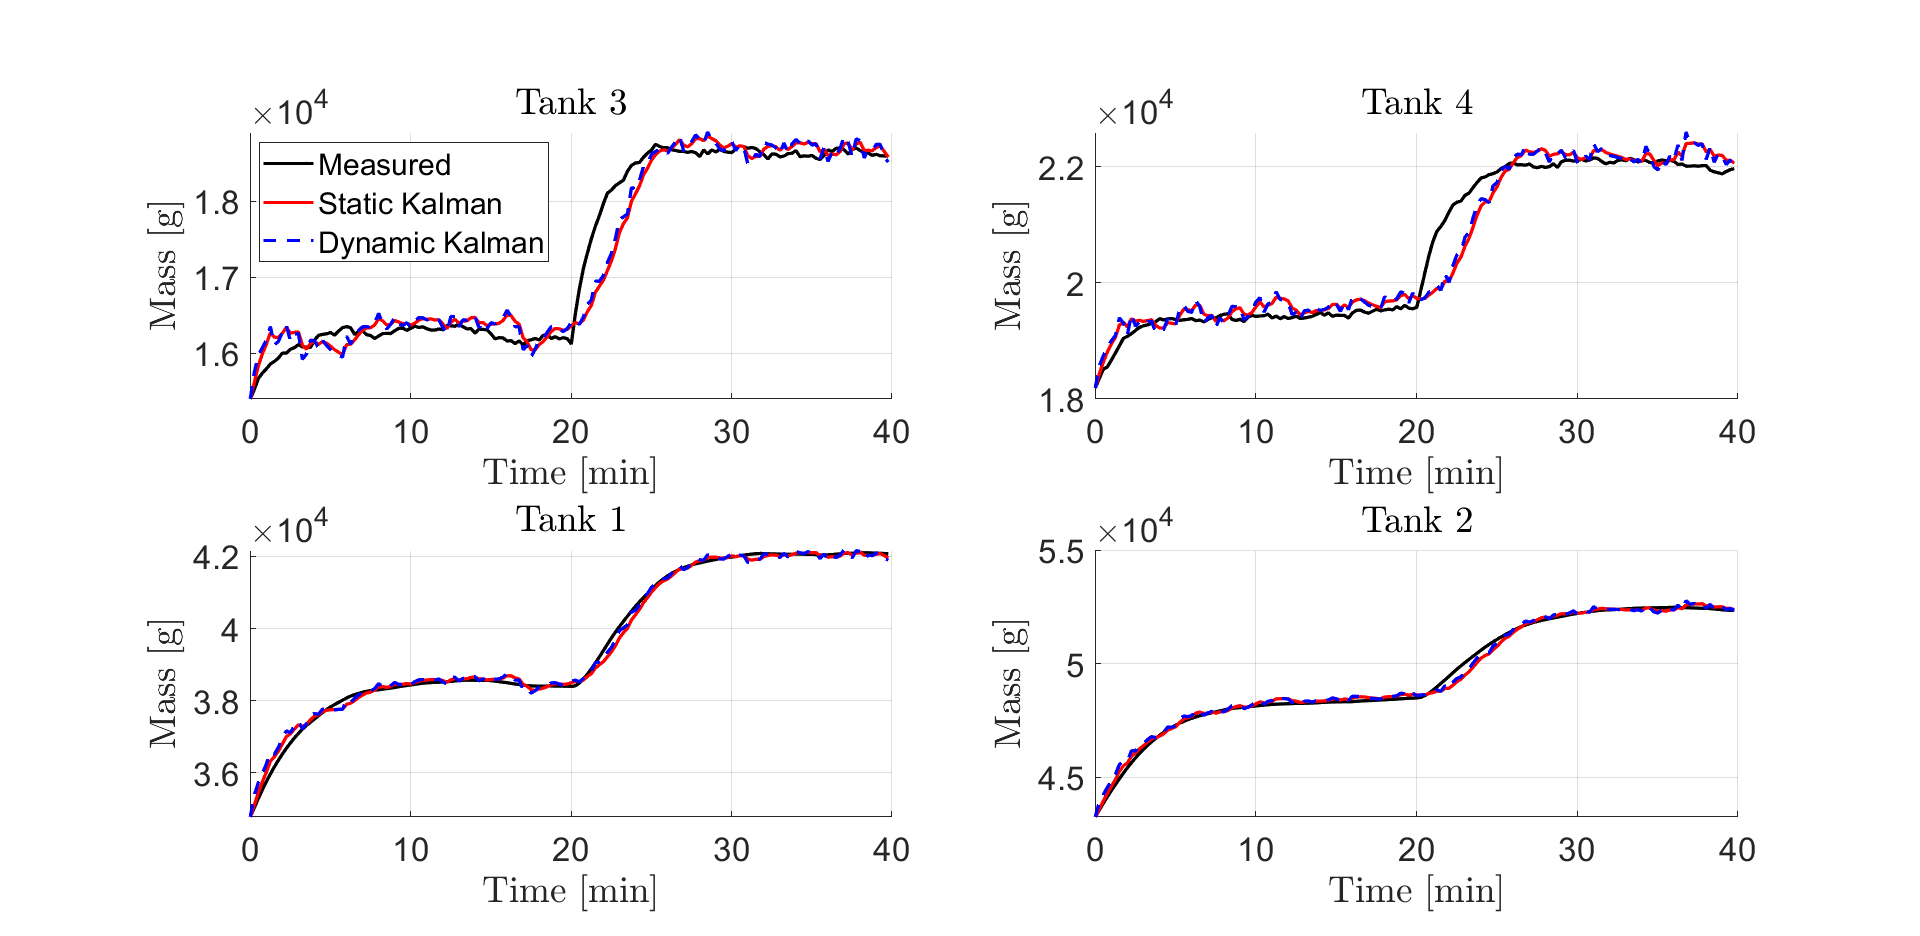
\includegraphics[width=1\textwidth]{Figures/Pr5.4_stoc_states.png}
    \caption{Kalman filter - Non-linear system - Stochastic model states}
    %\label{fig:Kalman_stoc_state_step}
\end{figure}
\begin{figure}[H]
    \centering
    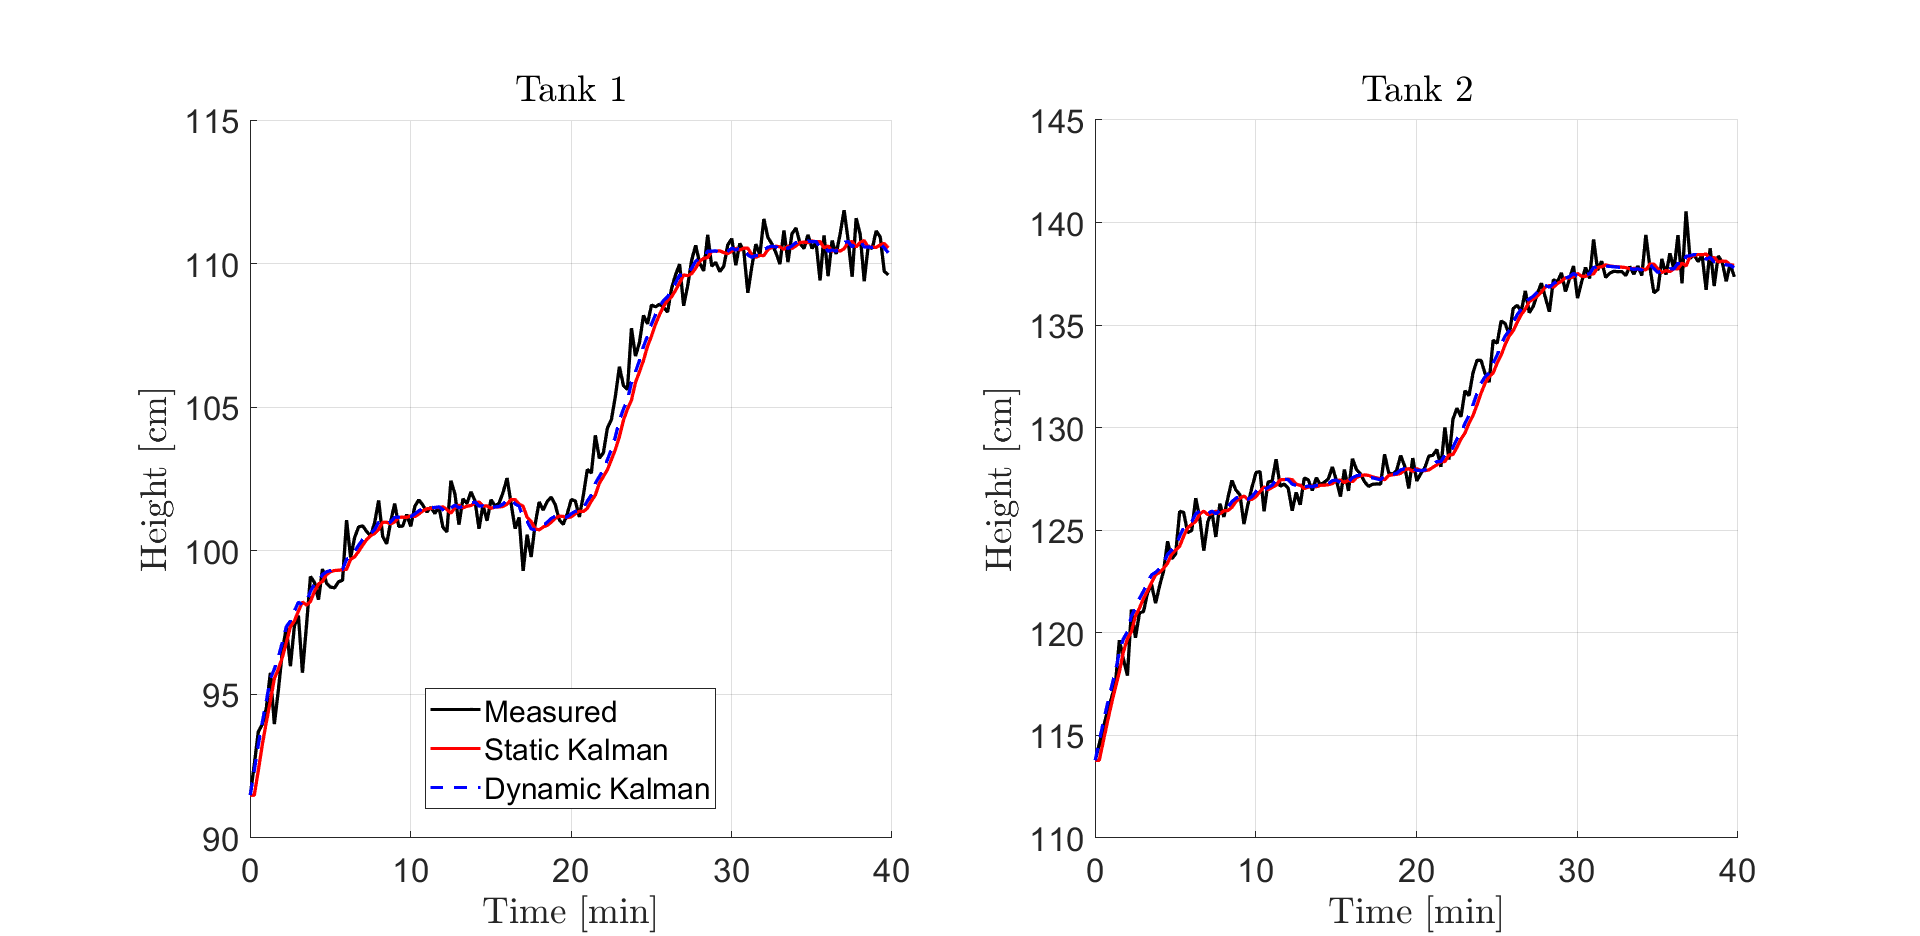
\includegraphics[width=1\textwidth]{Figures/Pr5.4_stoc_output.png}
    \caption{Kalman filter - Non-linear system - Stochastic model outputs}
    %\label{fig:Kalman_stoc_state_step}
\end{figure}
As seen, the difference between the Kalman filter performance on the linear and non-linear model is quite similar. However when the step on the disturbance have occurred, a constant offset (in the states) is seen which is due to the non-linearity's. 